\section{Dialogsystem für NPC-Trainer}\label{sec:dialogsystem-fur-npc-trainer}
In diesem Release wird das Spiel \textit{Monster Odyssey} um ein Dialogsystem erweitert. Damit kann der Nutzer Dialoge mit NPC-Trainern führen und gegebenenfalls Aktionen mit bestimmten NPC-Trainern tätigen.
Die Aktionen können sich je nach Situation beziehungsweise angesprochenem Trainer unterscheiden.
Beispielsweise kann der Nutzer ein Starter-Monster nach dem Gespräch mit dem Trainer Prof. Albert erhalten, seine eigenen Monster bei einer Krankenschwester in einem 'Moncenter' heilen oder Kämpfe mit bestimmten NPC-Trainern starten.
\subsection{Mockups}\label{subsec:mockups-dialogsystem}
In der Abbildung~\ref{fig: User and NPC-Trainer} befindet sich der Nutzer auf einem Spielfeld und ihm steht ein NPC-Trainer gegenüber. Wenn der Nutzer einem NPC-Trainer frontal zugewandt ist, kann nach Drücken der Interaktionstaste ein Dialog gestartet werden. Der Dialog wird anschließend von dem jeweiligen NPC-Trainer geführt und in der Abbildung~\ref{fig: Dialog User and NPC-Trainer} antwortet der NPC-Trainer mit einem Beispielsatz in einem Dialogfenster: „Hey there! Did you see Pikawatch in Route 100?“. In diesem Dialogfenster sieht der Nutzer den Namen des angesprochenen NPC-Trainers vor dem Satz und wird außerdem darauf hingewiesen, je nach Kontext mit dem nächsten Satz fortzufahren beziehungsweise den Dialog zu beenden, sobald die Interaktionstaste gedrückt wird.
\begin{figure}[H]
    \centering
    \begin{subfigure}[b]{0.4\textwidth}
        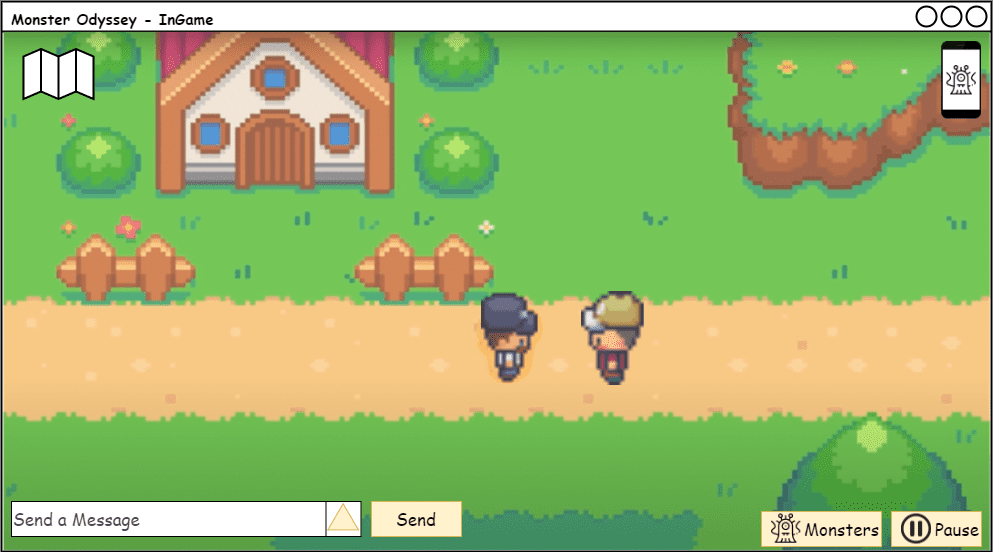
\includegraphics[width=\textwidth]{images/mockups/General/PlayerAndPlayer}
        \caption{Nutzer und NPC-Trainer voreinander}
        \label{fig: User and NPC-Trainer}
    \end{subfigure}
    \hfill
    \begin{subfigure}[b]{0.4\textwidth}
        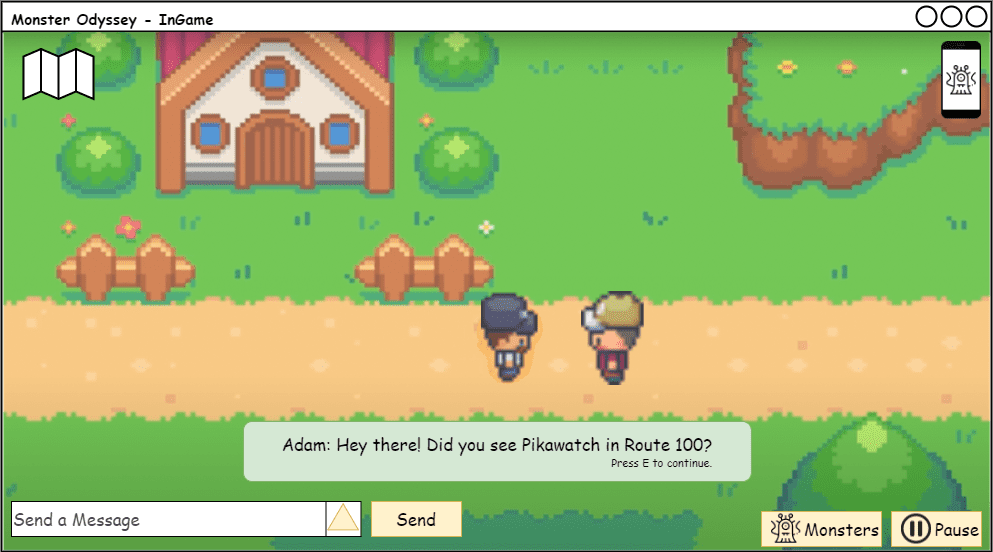
\includegraphics[width=\textwidth]{images/mockups/General/PlayerAndNPCMessage}
        \caption{Dialog zwischen Nutzer und NPC-Trainer}
        \label{fig: Dialog User and NPC-Trainer}
    \end{subfigure}
    \caption{Mockup: Starten eines Dialogs mit NPC-Trainer}
    \label{fig: Starten eines Dialogs mit NPC-Trainer}
\end{figure}
\subsection{Vergleich zwischen Mockups und Implementierung}\label{subsec:vergleich-zwischen-mockups-und-implementierung-dialogsystem}
In der Abbildung~\ref{fig: Vergleich: Anforderung Dialogsystem} sind verschiedene Unterschiede anzumerken. Bezüglich der Anforderung des Dialogsystems ist der Dialogbehälter deutlich größer als auf den Mockups wie in der Abbildung~\ref{fig: Mockup: Dialog zwischen Nutzer und NPC-Trainer}. Dies ist darauf zurückzuführen, dass einige Dialogtexte in den angebotenen Sprachen viel Platz in Anspruch nehmen. Außerdem ist die Schriftgröße der Anzeige zum Fortsetzen des Dialogs etwas größer formatiert, da dies für den Nutzer durch die Hervorhebung leichter zu identifizieren. Darüber hinaus ist der Trainername des angesprochenen Trainers in einem eigenen Behälter, über dem Dialogbehälter links liegend, vorzufinden. Somit werden der Text und der Name klar getrennt, um den Namen hervorzuheben. Der Namensbehälter wird in der Implementierung wie in der Abbildung~\ref{fig: Implementierung: Dialog zwischen Nutzer und NPC-Trainer} mit hellgrünem Hintergrund ausgestattet, damit Variabilität erzielt werden kann.

\begin{figure}[H]
    \centering
    \begin{subfigure}[b]{0.4\textwidth}
        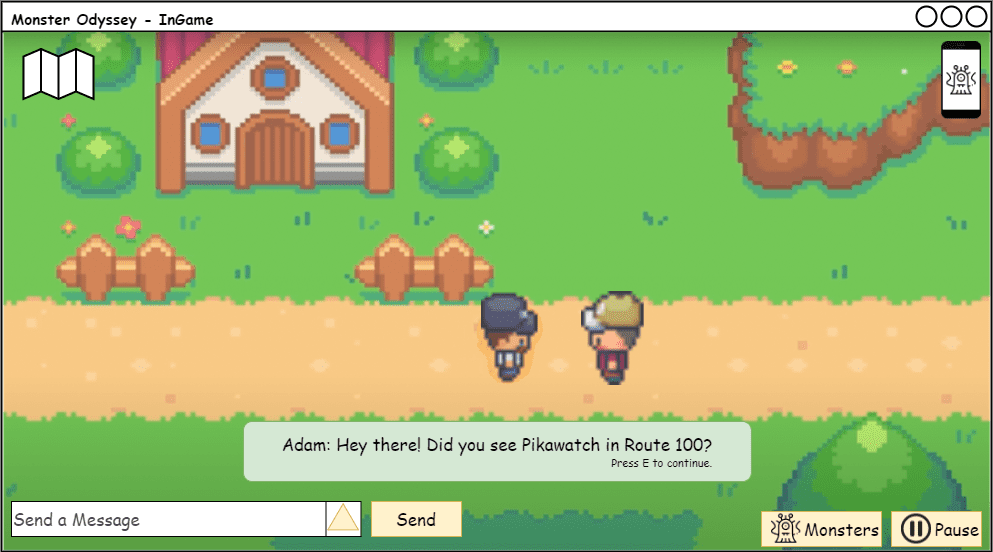
\includegraphics[width=\textwidth]{images/mockups/General/PlayerAndNPCMessage.png}
        \caption{Mockup: Dialog zwischen Nutzer und NPC-Trainer}
        \label{fig: Mockup: Dialog zwischen Nutzer und NPC-Trainer}
    \end{subfigure}
    \hfill
    \begin{subfigure}[b]{0.4\textwidth}
        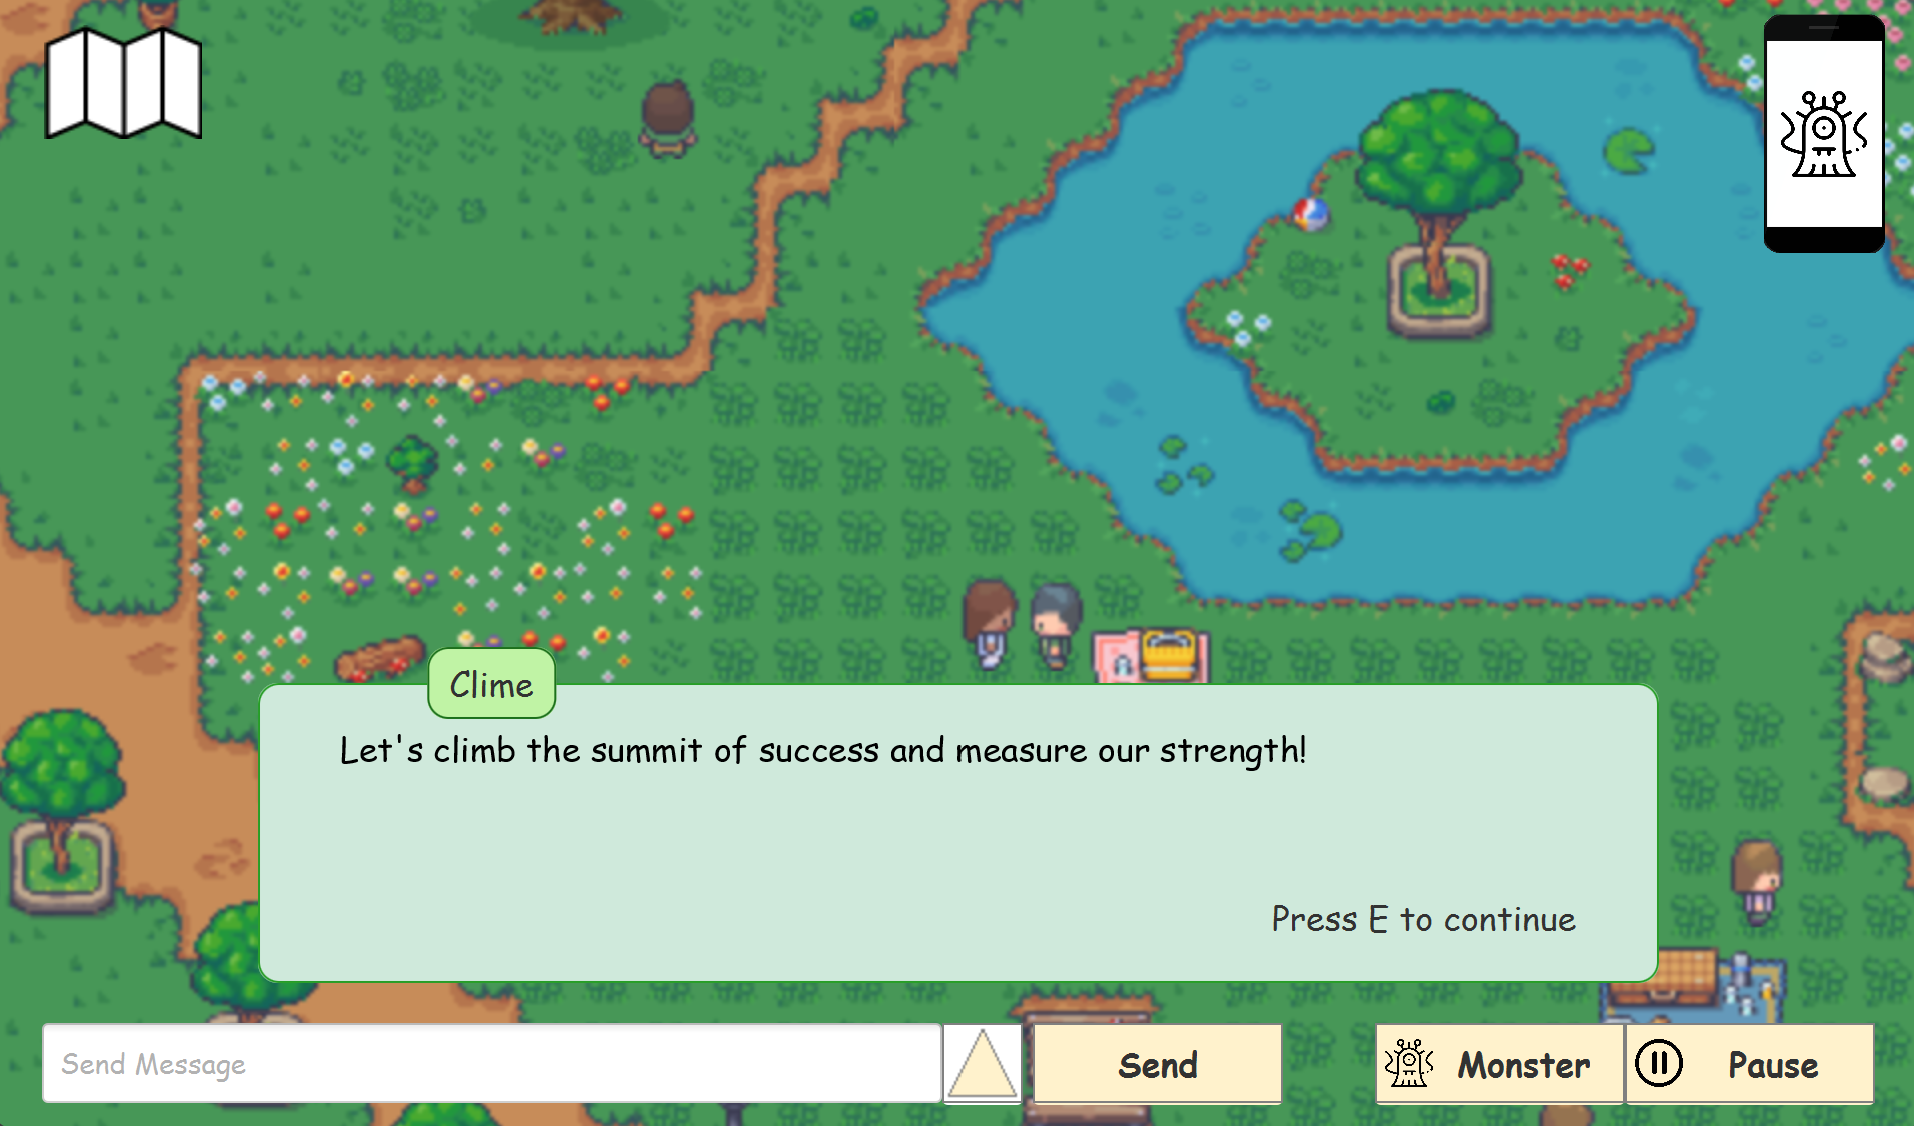
\includegraphics[width=\textwidth]{images/implementation/General/Implementierung Dialog.png}
        \caption{Implementierung: Dialog zwischen Nutzer und NPC-Trainer}
        \label{fig: Implementierung: Dialog zwischen Nutzer und NPC-Trainer}
    \end{subfigure}
    \caption{Vergleich: Anforderung Dialogsystem}
    \label{fig: Vergleich: Anforderung Dialogsystem}
\end{figure}